\documentclass{article}
\usepackage{v-problem}
\vgeometry

\newcommandx*\varea[3][1=solid, 2=3,3=-2.75, usedefault=@]{
	
	\tzcoors(3,1.5)(A)(5,2)(B)(5.5,3)(C)(4.5,4)(D)(2.5,3)(E);
	\tztos[#1]<#2, #3>
		(A)[out=-30,in=210]
		(B)[out=30,in=-90]
		(C)[out=90,in=-30]
		(D)[out=150,in=80]
		(E)[out=-90,in=150]
		(A);
}
\usetikzlibrary{fadings}

\begin{document}
\vtitle[ROTATION]

\def\pn{02}
\def\exam{JEE}
\def\year{2019}
\def\gdrive{https://drive.google.com/drive/folders/1PW0S7WBkzOopRpxHwUzqiTANITatoL9H?usp=share_link}

\def\question{
A thin circular plate of mass $M$ and radius $R$ has its density varying as $\rho(r)=\rho_0 r$ with $\rho_0$ as constant and $r$ is the distance from its center. The moment of inertia of the circular plate about an axis perpendicular to the plate and passing through its edge is $I=aMR^2$. The value of the coefficient $a$ is
}

\def\option{
\begin{tasks}(2)
\task $\dfrac{1}{2}$
\task $\dfrac{3}{5}$
\task $\dfrac{8}{5}$
\task $\dfrac{3}{2}$
\end{tasks}
}

\vspace*{\fill}
\begin{tikzpicture}
	\node[qnumber] (n) at (0, 0)[scale=2] {$\pn.$};
	\node[question] (q) [right=2mm of n.east] {\question};
	\tzline[divider]<-0.125, 0> (q.north west)(q.south west);
	\node[format] (f) at  (q.south east){[\exam \quad \year]};
\end{tikzpicture}	
\vspace*{\fill}

\begin{center}
\begin{tikzpicture}
	\tzcircle[shading=radial, inner color=black!80, outer color=black!30](0, 0)(1.75)
	\tzring*[pattern=crosshatch](0, 0)(1.5)(0, 0)(1.35)
	\tzline[->](0, 0)(1.35, 0){$r$}[mb]
	\tzdot*(0, 0)
\end{tikzpicture}
\end{center}

\vspace*{\fill}

\begin{tikzpicture}
\node[minimum width=1cm](n) at (0, 0){}; 
\node[option, anchor=west] at (n.east){\option};
\end{tikzpicture}
\vspace*{\fill}
\pagebreak
\vtitle[\texttt{Solution}]
\begin{center}
\begin{tikzpicture}
	\tzcircle[shading=radial, inner color=black!80, outer color=black!30](0, 0)(1.75)
	\tzring*[pattern=crosshatch](0, 0)(1.5)(0, 0)(1.35)
	\tzline[->](0, 0)(1.35, 0){$r$}[mb]
	\tzdot*(0, 0)
	%\tzline(-1.75,-2.5)(-1.75, 2.5) {$Y'$}[a]
	%\tzarc[->,PINKA](-1.75,2)(60:300:0.5 and 0.2)
	\tzline[->](0, 0, 0)(4, 0, 0){$X$}[r]
	\tzline[->](0, 0, 0)(0, 4, 0){$Y$}[a]
	\tzline[->](0, 0, 0)(0, 0, 5){$Z$}[b]
	\tzline[->](-1.75, 0, -5)(-1.75, 0, 5){$Z'$}[b]
\end{tikzpicture}
\end{center}
\vspace*{\fill}
\begin{align*}
I_{Z'} &= I_Z + MR^2 &&\texttt{parallel axis theorem}\\
\end{align*}
\pagebreak

\begin{align*}
I_{Z'} &= I_Z + MR^2\\
aMR^2  &= I_Z + MR^2\\
\left(a-1\right)R^2M &=I_Z\\
\left(a-1\right)R^2\int_0^R\d{m} &= \int_0^R \d{m}r^2 \\
\left(a-1\right)R^2\int_0^R\left(\rho 2\pi r \d{r}\right) &= \int_0^R\left(\rho 2\pi r \d{r}\right) r^2 \\
\left(a-1\right)R^2\int_0^R\left(\rho_0 r 2\pi r \d{r}\right) &= \int_0^R\left(\rho_0 r 2\pi r \d{r}\right) r^2 \\
\left(a-1\right)2\rho_0 \pi R^2\int_0^R r^2 \d{r}  &= 2\rho_0 \pi \int_0^R r^4 \d{r}\\
\left(a-1\right)2\rho_0\pi\dfrac{R^5}{3} &= 2\rho_0\pi \left(\dfrac{R^5}{5}\right) \\
a &= \dfrac{3}{5} + 1\\
a &= \dfrac{8}{5}\ans
\end{align*}

\pagebreak

\vspace*{\fill}
\begin{center}
	\fbox{\qrcode[height=2cm]{\gdrive}}
\end{center}
\vspace*{\fill}

\pagebreak
\vspace*{\fill}
\begin{center}
\begin{tikzpicture}
	\tzline(-0.5, 0)(6, 0)
	
	\tzline+[line width=2mm, black!45](0.5, 0)(0, 5){\texttt{Imagination}}[scale=0.5, b=5cm]
	\foreach \h/\t in {1/Reading, 2.5/Making, 4/Making-mistakes}{
		\tzline+[line width=2mm](\h + 1, 0)(0, \h){\texttt{\t}}[b=\h cm, scale=0.5]
	}
\end{tikzpicture}
\end{center}
\vspace*{\fill}

\pagebreak
\vspace*{\fill}
\begin{center}
\begin{tikzpicture}
	[thick]
	
	\tzlines(0, 0)(0.5, 1)(1, 0.5)(1.5, 1.5)(2, 1)(2.5, 2)(6, 2){\texttt{I know everything}}[ma, scale=0.7];
	\tzlines[dashed]<2.5, 2>(0, 0)(0.5, 1)(1, 0.5)(1.5, 1.5)(2, 1)(2.5, 2)(6, 2){\texttt{I know e...}}[ma, scale=0.7];
	\tzlines[dashed]<5, 4>(0, 0)(0.5, 1)(1, 0.5)(1.5, 1.5)(2, 1)(2.5, 2);
\end{tikzpicture}
\end{center}
\vspace*{\fill}

\pagebreak
\vspace*{\fill}
\begin{center}
\begin{tikzpicture}
	[thick]
	\tzcircle(0, 0)(1)
	\tznode(0, -1.2){\texttt{tension in becoming someone}}[b, scale=0.65]
	\begin{scope}[scale=0.65]
		\varea
	\end{scope}
	\tznode(4.5, -1.2){\texttt{relaxation in being yourself}}[b, scale=0.65]
\end{tikzpicture}
\end{center}
\vspace*{\fill}

\end{document}
